\documentclass[11pt]{exam}

\oddsidemargin=0.25truein \evensidemargin=0.25truein
\topmargin=-0.5truein \textwidth=6.0truein \textheight=8.75truein

\usepackage{comment}
\usepackage{verbatim}
\usepackage{booktabs}
\usepackage{graphicx}
\usepackage{hyperref}
\urlstyle{rm}   % change fonts for url's (from Chad Jones)
\hypersetup{
    colorlinks=true,        % kills boxes
    allcolors=blue,
    pdfsubject={ECON-UB233, Macroeconomic foundations for asset pricing},
    pdfauthor={Dave Backus @ NYU},
    pdfstartview={FitH},
    pdfpagemode={UseNone},
%    pdfnewwindow=true,      % links in new window
%    linkcolor=blue,         % color of internal links
%    citecolor=blue,         % color of links to bibliography
%    filecolor=blue,         % color of file links
%    urlcolor=blue           % color of external links
% see:  http://www.tug.org/applications/hyperref/manual.html
}

\renewcommand{\thefootnote}{\fnsymbol{footnote}}
\newcommand{\var}{\mbox{\it Var\/}}

%\printanswers

% document starts here
\begin{document}
\parskip=\bigskipamount
\parindent=0.0in
\thispagestyle{empty}
{\large ECON-UB 233 \hfill Dave Backus @ NYU}

\bigskip\bigskip
\centerline{\Large \bf Lab Report \#8:  Bond Pricing}
\centerline{(Started: April 11, 2012; Revised: \today)}

\bigskip
{\it Due at the start of class.
You may speak to others, but whatever you hand in should be your own work.}

\begin{questions}

\begin{solution}
Answers follow.  See Matlab code at the end for calculations.
\end{solution}

%-----------------------------------------------------------------------
\question (estimating parameters for the Vasicek model)
Consider the Vasicek model, which for our purposes will
be the pricing kernel
\begin{eqnarray*}
    \log m_t &=& \delta + \sum_{j=0}^\infty a_j w_{t-j}
\end{eqnarray*}
with parameters $(\delta, a_0, a_1, \varphi)$
and $a_{j+1} = \varphi a_j$ for $j\geq 1$.
This is, of course, the ARMA(1,1) version of our infinite moving average.

We'll use the data in Table 3 of

\url{http://pages.stern.nyu.edu/~dbackus/233/BFMW_JFE_01.pdf},

specifically the properties of forward rates,
to estimate the parameters of the model.
The same table was distributed in class with the notes on
bond pricing.
And remember:  the data are reported as annual percentages,
but the time interval here is monthly.

%
\begin{parts}
\part What parameter values reproduce the reported
standard deviation and autocorrelation of the short rate
(the forward rate of maturity 0)?

\part Choose $a_0$ to reproduce the
mean difference between forwards of maturity $n=60$ (5 years)
and $n=0$.

\part Given the other parameters, what value of $\delta$
reproduces the mean short rate?

\part What do your parameter values imply for the mean difference
between forwards of maturity $n=120$ (10 years) and $n=0$?
$n=24$ (2 years)?

\part Given your parameter values, how does the standard deviation
of the $n$-period forward rate vary with $n$?
How do your numbers compare to those in the table?

\part How would you summarize the differences between the model's implications
and the evidence?
\end{parts}

\begin{solution}
The idea here is that this model gives us a rough approximation
of what we see in the data, but there are a number
of dimensions it misses on.
That's ok, it's a simple model, but this process of identifying weaknesses
leads over time to better models.
\begin{parts}
\part The short rate $f^0_t$ is
\begin{eqnarray*}
    - f^0_t &=& \log E_t m_{t+1}
            \;\;=\;\; \delta + a_0^2/2 + \sum_{j=0}^\infty a_{1} \varphi^j w_{t-j} .
\end{eqnarray*}
This has mean $\delta + a_0^2/2$, variance $a_1^2/(1-\varphi^2)$,
and autocorrelation $\varphi$.
With the numbers we're given, that implies $\varphi = 0.959$.
$a_1 = -0.645 \times 10^{-3}$,
and $\delta = (6.683/1200) - a_0^2/2 $.
\part Roughly $a_0 = 0.1243$.  Any sign, as long as it's the opposite of $a_1$.
\part Now that we have $a_0$, we set $\delta = (6.683/1200) - a_0^2/2 = -0.0133 $.
\part As we saw in class, we don't get all maturities right.
Here we hit $f^{60}$ by design.  For some other maturities

\begin{center}
\begin{tabular}{lcc}
\toprule
Maturity &  Model & Data \\
\midrule
$ n=36$    &  1.738  & 1.815     \\
$ n=120$   &  2.186  & 2.175    \\
\bottomrule
\end{tabular}
\end{center}
The numbers here have been multiplied by 1200 to make
them comparable to the table.
You can see we're a little low with the first one and (slightly)
high with the second.
\item The moving average coefficients for maturity $n$
are $ a_{n+1+j} = \varphi^{n+j} a_1 $ for $j\geq 0$.
That means the variance declines with maturity:
\begin{eqnarray*}
    \mbox{Var}(f^n) &=& \varphi^{2n} \mbox{Var}(f^0) .
\end{eqnarray*}
For the standard deviation, we take the square root.
That leads to the following comparison of model (line) and data (asterisks):

\begin{center}
%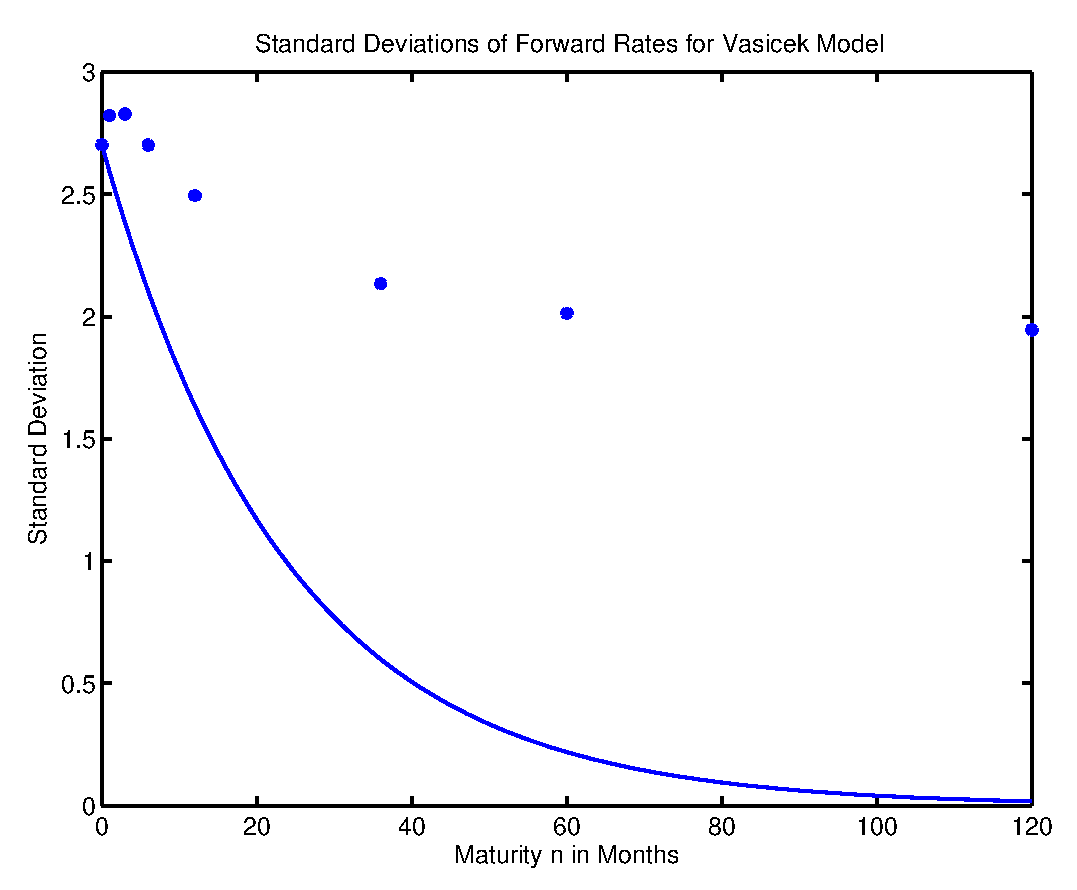
\includegraphics[width=4in]{../Matlab/hw8q1e.eps}
\end{center}

It's evident here that the model generates too little variation in long
forward rates.  That's a standard problem.
We could mitigate it by increasing the value of $\varphi$,
but that affects the model in other dimensions.

\part Lots of work left to do.  The standard deviation
of long rates is probably the biggest issue we've seen.

\end{parts}
\end{solution}

%-----------------------------------------------------------------------
\question (another affine model)
Consider the bond pricing model characterized by
\begin{eqnarray*}
    \log m_{t+1} &=& - (\lambda_0 + \lambda_1 x_t)^2/2  - x_t  +
                        (\lambda_0 + \lambda_1 x_t) w_{t+1} \\
         x_{t+1} &=& (1-\varphi) \delta + \varphi x_t + \sigma w_{t+1} .
\end{eqnarray*}
This is sometimes referred to as an ``essentially affine model,''
but the reasons for that escape me.
It is, however, a third convenient example of an affine model ---
in addition to Vasicek and CIR.

\begin{parts}
\part  What is the one-period bond price?
What role does the term  $-(\lambda_0 + \lambda_1 x_t)^2/2$ play?

\part Suppose bond prices take the form
\begin{eqnarray*}
    \log q^n_{t} &=& A_n + B_n x_t .
\end{eqnarray*}
What are the recursions that generate $(A_{n+1}, B_{n+1})$ from
$(A_{n}, B_{n})$?
What initial values $(A_{0}, B_{0})$ would you use?

\part Suppose $\lambda_0$ is given to you.
Using the same logic as the previous question,
use features of the short rate $f^0$ and the five-year forward rate
$f^{60}$ to determine the other parameters, $(\varphi, \sigma, \lambda_1)$.

\part Plot mean forward rates $E(f^n)$ versus maturity $n$.
Comment on any differences between the model and the evidence.
\end{parts}


\begin{solution}
This is another ``affine'' model, one that's been widely used
because it gives us a lot of flexibility over the connection
between term premiums and the state variable $x_t$.
The mechanics follow the usual route, so what follows is
somewhat terse.
\begin{parts}
\part The short rate is
\begin{eqnarray*}
    f^0_t &=& x_t .
\end{eqnarray*}
The first term in the pricing kernel cancels out with the ``variance over two'' term.

\part This will take you some work, and I've reverted to standard notation,
but the answer is
\begin{eqnarray*}
    A_{n+1} &=& A_n + B_n [(1-\varphi) \delta + \sigma \lambda_0] + (B_n\sigma)^2/2 \\
    B_{n+1} &=& B_n (\varphi+\sigma\lambda_1) - 1 .
\end{eqnarray*}
We start, as always, with $A_0 = B_0 = 0$.

\part Same as usual.  Here we have two ways to hit the mean forward rate curve,
$\lambda_0$ and $\lambda_1$.

\part Looks similar to the Vasicek model.  See Matlab program for details.

\end{parts}
\end{solution}



\end{questions}

\vfill \centerline{\it \copyright \ \number\year \
NYU Stern School of Business}

%\end{document}

\pagebreak
Matlab program:
\verbatiminput{../Matlab/hw8_s12.m}

\end{document}


%  EXTRA STUFF


